%%%%%%%%%%%
%% CARLA %%
%%%%%%%%%%%

\subsection{CARLA}

CARLA (Car Learning to Act) (\cite{dosovitskiy2017carla}) is an open-source simulator for autonomous driving research. It is designed to support development, training, and validation of autonomous urban driving systems. CARLA is flexible and realistic, providing a variety of environmental conditions and vehicle models for testing. Key features of CARLA include:

\begin{itemize}
\item Realistic rendering of urban environments, including a variety of pre-designed maps as well as tools for creating custom maps.
\item A rich set of sensors, including lidar, cameras, GNSS, radar, and more.
\item Full control over environmental conditions, such as weather and lighting.
\item Support for a variety of traffic scenarios, including other vehicles, pedestrians, and various traffic rules.
\item A Python API for controlling vehicles, sensors, and the environment, which can be used to integrate CARLA with machine learning frameworks.
\end{itemize}

CARLA is built on a scalable client-server architecture. The server side encompasses all aspects of the simulation process, including sensor rendering, physics computations, and updates to the world-state and its actors, among other responsibilities. For the sake of producing realistic results, it is recommended that the server is operated with a dedicated GPU, particularly when it is used in machine learning applications.


\begin{figure}[H]
\centering
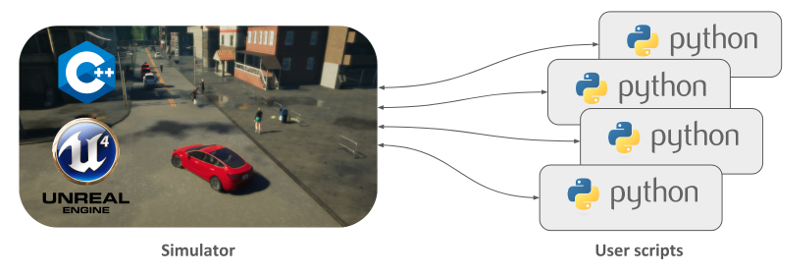
\includegraphics[width=1\linewidth]{Figures/Methods/carla_modules.png}
\caption{CARLA client-server architecture, where the Simulator is provided on the server side, and scripts can control the simulator on the client side}
\label{fig:carla_modules}
\end{figure}

The client-side of the architecture comprises numerous client modules, each controlling the logic of the actors in the scene and determining the world's conditions. The interaction between the server and client is facilitated by the CARLA API, available in Python or C++, which serves as an intermediary layer. This API is continually updated to offer new functionalities, enhancing the overall capabilities of the CARLA simulator.

The basic structure of CARLA can be summarised as:

\begin{itemize}
\item \textbf{Traffic Manager:} This is an integrated system in CARLA that manages the control of all vehicles excluding the one used for learning. It functions as a conductor to mimic realistic behaviours in urban-like environments.
\item \textbf{Sensors:} These are essential components for vehicles to gather information about their environment. In CARLA, sensors are a unique type of actor attached to the vehicle, and the data they collect can be accessed and stored for convenience. CARLA supports a range of sensors, including cameras, radars, lidars, and more.
\item \textbf{Recorder:} This tool allows for the step-by-step recreation of a simulation for every actor in the world. It provides access to any moment in the timeline at any location, making it a powerful tracing tool.
\item \textbf{ROS Bridge and Autoware Implementation:} In the pursuit of universal applicability, the CARLA project actively seeks to integrate the simulator within other learning environments.
\item \textbf{Open Assets:} CARLA provides various maps for urban settings, complete with control over weather conditions and a blueprint library containing a broad range of actors. These assets can be customized, and new ones can be created following simple guidelines.
\item \textbf{Scenario Runner:} To streamline the learning process for vehicles, CARLA provides a series of routes that describe different situations to iterate on. These routes also form the foundation for the CARLA challenge, an open competition for everyone to test their solutions and aim for a spot on the leaderboard.
\end{itemize}

\subsection{Spawn points}

